
The possibilities for oscillations in two and higher dimensions are incredibly richer. The simplest of these possibilities is the so-called {\bfseries isotropic harmonic oscillator}, for which the restoring force is proportional to the displacement from equilibrium, with same spring constant in all directions such that, $\vec{F} = -k\vec{r}$. A 2D case is a mass with four springs pointing towards each of the cardinal directions. A 3D example is a proton or neutron inside a nucleus.

The equation of motion for the 2D case with the same force constant $k$ is, $\ddot{x} = -\omega^2x$ and $\ddot{y} = -\omega^2y$, where $\omega = \sqrt{k/m}$. The solutions have already been determined from the last section,

\begin{gather*}
    x(t) = A_x cos(\omega t - \delta_x) \\
    y(t) = A_y cos(\omega t - \delta_y) 
\end{gather*}

\noindent where the four constants are determined by the initial conditions of the problem. The motion of this system is described by the choice of these variables. See figure \ref{fig:Osc2D_examples}.

The other type of multi-dimensional oscillator is the {\bfseries anisotropic oscillator}, where the restoring force components are proportional to the displacement but with different force constants $k_x$, $k_y$, and $k_z$.

Similar to the previous example of an isotropic harmonic oscillator, we receive the solutions,

\begin{gather*}
    x(t) = A_x cos(\omega_x t - \delta_x) \\
    y(t) = A_y cos(\omega_y t - \delta_y) 
\end{gather*}

\noindent however, note $\omega_x = \sqrt{k_x/m}$ and $\omega_y = \sqrt{k_y/m}$. Since $k_x \neq k_y$, $\omega_x \neq \omega_y$. This result gives the asymmetric-looking solutions shown in figure \ref{fig:Osc2D_anisotropic}.

\begin{figure}[h]
    \centering
    \begin{subfigure}[t]{0.3\textwidth}
        \centering
        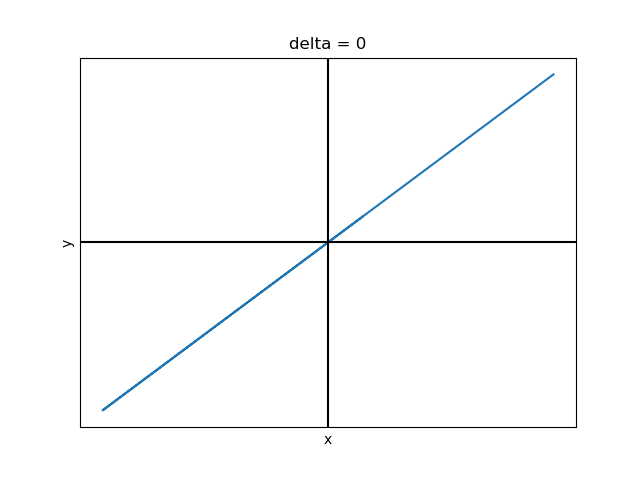
\includegraphics[width=4.85cm]{Classical_Mechanics/2.11-2d-osc/Osc2D_delta0.png}
        \caption{$\delta = 0$}
    \end{subfigure}
    ~ 
    \begin{subfigure}[t]{0.3\textwidth}
        \centering
        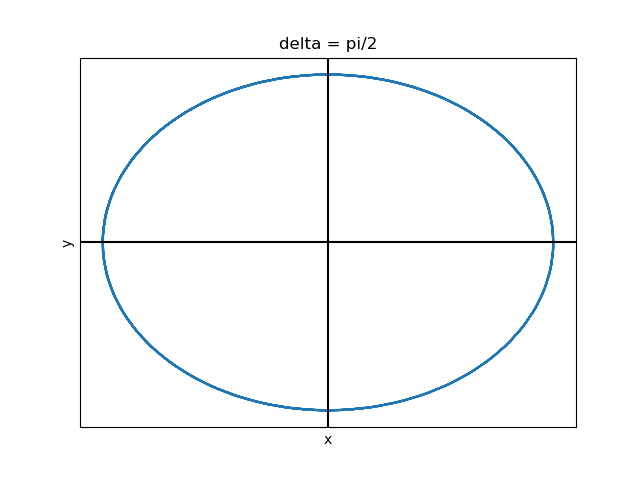
\includegraphics[width=4.85cm]{Classical_Mechanics/2.11-2d-osc/Osc2D_deltapi2.png}
        \caption{$\delta = \frac{\pi}{2}$}
    \end{subfigure}
    ~
    \begin{subfigure}[t]{0.3\textwidth}
        \centering
        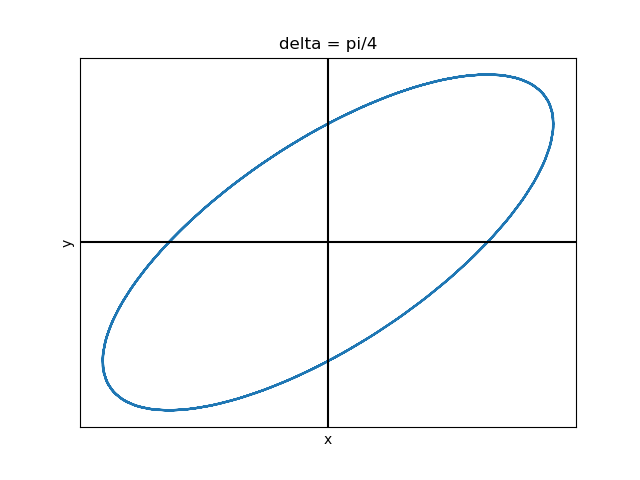
\includegraphics[width=4.85cm]{Classical_Mechanics/2.11-2d-osc/Osc2D_deltapi4.png}
        \caption{$\delta = \frac{\pi}{4}$}
    \end{subfigure}
    \caption{Plots $x$ vs $y$ in 2D oscillators using constants $A_x = A_y = \omega = 1$ and $\delta$ given below each plot.}
    \label{fig:Osc2D_examples}
\end{figure}

\begin{figure}[h]
    \centering
    \begin{subfigure}[t]{0.4\textwidth}
        \centering
        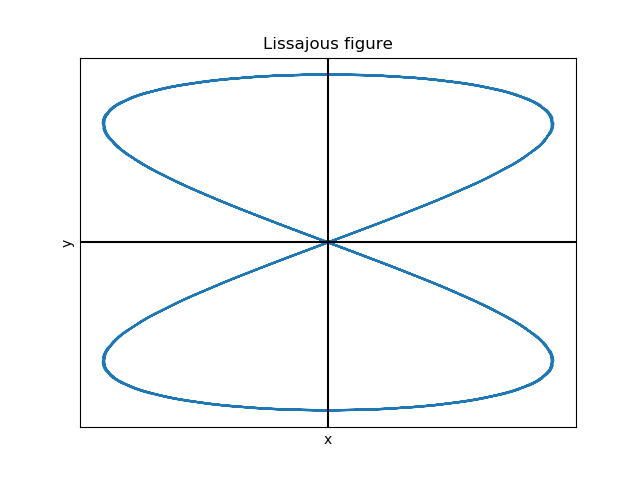
\includegraphics[width=6.5cm]{Classical_Mechanics/2.11-2d-osc/Osc2D_wx2wy.png}
        \caption{When $\frac{\omega_x}{\omega_y}$ is rational ($\frac{2}{1}$ in this example), we find the Lissajous figure. The amount of turns depends on the angular frequency $\omega$.}
    \end{subfigure}
    ~ 
    \begin{subfigure}[t]{0.4\textwidth}
        \centering
        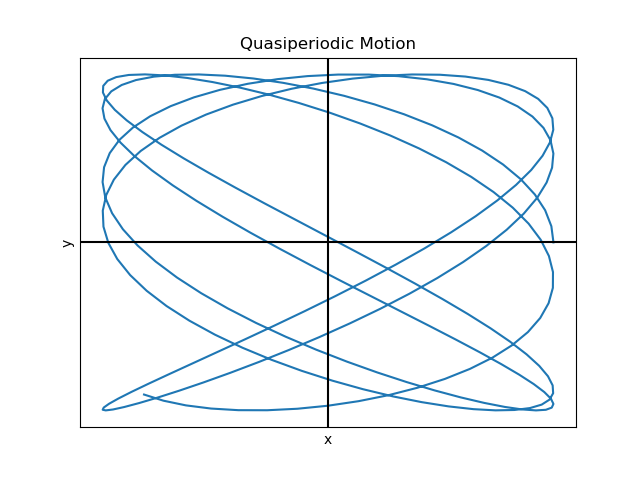
\includegraphics[width=6.5cm]{Classical_Mechanics/2.11-2d-osc/Osc2D_quasi.png}
        \caption{If $\frac{\omega_x}{\omega_y}$ is irrational ($\frac{\sqrt{2}}{1}$ in this example), the motion is said the be {\bfseries quasiperiodic}. Both $x$ and $y$ are periodic but the motion as a whole is not.}
    \end{subfigure}
    \caption{Plots of a 2D anisotropic oscillator}
    \label{fig:Osc2D_anisotropic}
\end{figure}
